\RequirePackage{fix-cm}
\documentclass[oneside, a4paper]{book}
\usepackage[a4paper,width=150mm,top=25mm,bottom=25mm,bindingoffset=6mm]{geometry}

% Required for inserting images
\usepackage{eso-pic,graphicx}
% misc
\usepackage{caption}
\DeclareCaptionType{equ}[][]
%\captionsetup[equ]{labelformat=empty}
\usepackage{subcaption}
\usepackage{multicol}
\usepackage{float}
\usepackage{adjustbox} % oversized table

% appendix
\usepackage[toc]{appendix}

% Default font to sans serif
\renewcommand{\familydefault}{\sfdefault}
\RequirePackage[T1]{fontenc} 
\RequirePackage[tt=false, type1=true]{libertine} 
\RequirePackage[varqu]{zi4} 
% \RequirePackage[libertine]{newtxmath}

% chapters and headers
\usepackage[Conny]{fncychap}

\usepackage{fancyhdr}
\pagestyle{fancy}
\renewcommand{\headrulewidth}{0.1pt}
\renewcommand{\chaptermark}[1]{\markboth{\MakeUppercase{\textsf{{#1}}}}{}}
\renewcommand{\sectionmark}[1]{\markright{\MakeUppercase{\textsf{\thesection\ #1}}}{} }

% section styling
\usepackage{titlesec}

% algorithms
\usepackage{algorithm}
\usepackage{algpseudocode}

% theorems and definitions
\usepackage{amsthm}
\newtheorem{definition}{Definition}

% better tables
\usepackage{tabu}

% FAT FONTS
\usepackage{bm} % bold fonts in math mode
\newcommand\fat[1]{{\boldmath{\textbf{#1}}}}
\newcommand\emphasis[1]{{\scshape\bfseries#1}}

% mathematical fonts and graphics
\usepackage{mathtools}
\usepackage{xfrac} % sfrac for diagonal slashes in fractions
\usepackage{amsfonts} % math fonts
\usepackage{amssymb} % more math symbols (supsetneq etc.)
\usepackage{dbnsymb}
\usepackage{dsfont} % math fonts
\usepackage{bbm} % mathbb fonts
\usepackage{mathrsfs} % fancy swirly font
\usepackage{gensymb} % degree sign

% draw graphs
\usepackage[inline]{asymptote}
\usepackage{qtree}
\usepackage{tikz}
\usetikzlibrary{calc}

% nicer fractions
\usepackage{xfrac}
% cancel terms
\usepackage{cancel}

% units
\usepackage{siunitx}

% plots
\usepackage{pgfplots}
\usepackage{pgfplotstable}
\usepgfplotslibrary{external}
\usepgfplotslibrary{patchplots}
\usepgfplotslibrary{groupplots}
\pgfplotsset{compat=1.18} 
\tikzexternalize[prefix=tikz,optimize=false]

% define the Spectral_r color scheme
\usepackage[table, dvipsnames]{xcolor}
\definecolor{Spectral0}{RGB}{158, 1, 66}
\definecolor{Spectral1}{RGB}{213, 62, 79}
\definecolor{Spectral2}{RGB}{244, 109, 67}
\definecolor{Spectral3}{RGB}{253, 174, 97}
\definecolor{Spectral4}{RGB}{254,224,139}
\definecolor{Spectral5}{RGB}{255,255,191}
\definecolor{Spectral6}{RGB}{230,245,152}
\definecolor{Spectral7}{RGB}{171,221,164}
\definecolor{Spectral8}{RGB}{102,204,204}
\definecolor{Spectral9}{RGB}{50,136,189}
\definecolor{Spectral10}{RGB}{94,79,162}
\pgfplotsset{
  colormap={Spectral_r}{
    rgb255(0cm)=(94,79,162)         % 0.0
    rgb255(1cm)=(50,136,189)        % 0.1
    rgb255(2cm)=(102,204,204)       % 0.2
    rgb255(3cm)=(171,221,164)       % 0.3
    rgb255(4cm)=(230,245,152)       % 0.4
    rgb255(5cm)=(255,255,191)       % 0.5
    rgb255(6cm)=(254,224,139)       % 0.6
    rgb255(7cm)=(253,174,97)        % 0.7
    rgb255(8cm)=(244,109,67)        % 0.8
    rgb255(9cm)=(213,62,79)         % 0.9
    rgb255(10cm)=(158,1,66)         % 1.0
    }
}


% get width of given text
\usepackage{calc}

% define a horizontal spacer
\newcommand\horizontalspacer[0]{\vspace{5pt}\noindent\textcolor{lightgray}{\rule{\textwidth}{1mm}}
\vspace{5pt}}

% clickable links
\usepackage{hyperref}
\hypersetup{
    colorlinks,
    citecolor=black,
    filecolor=black,
    linkcolor=black,
    urlcolor=black
}
\renewcommand{\itemautorefname}{Item}
% fancy boxes
\usepackage{fancybox}
\newcommand{\equationnamed}[2]{%
  \setlength{\fboxsep}{2pt} % padding inside box
  \setlength{\fboxrule}{0.01pt}
  \begin{center}
    \begin{minipage}{\textwidth}
      \begin{center}\textsc{#1}\end{center}
      #2
    \end{minipage}
  \end{center}
}
\newcommand{\equationnamedbox}[2]{%
  \setlength{\fboxsep}{5pt} % padding inside box
  \setlength{\fboxrule}{0.01pt}
  \begin{center}
    \fbox{
      \begin{minipage}{0.4\textwidth}
        \begin{center}\emphasis{#1}\end{center}
        #2
      \end{minipage}
    }
  \end{center}
}

% labels to enum items
\usepackage{enumitem}

\usepackage{array}

% make empty lines skip
% \usepackage{parskip}

% include pdfs 
\usepackage{pdfpages}

% code
\usepackage{minted}
\usepackage{listings}

% ~~~~~~~~~ TYPESETTING AND OTHER MACROS ~~~~~~~~~~~~~~~~~~~~~

\newenvironment{absolutelynopagebreak}
  {\par\nobreak\vfil\penalty0\vfilneg
   \vtop\bgroup}
  {\par\xdef\tpd{\the\prevdepth}\egroup
   \prevdepth=\tpd}

% ~~~~~~~~~ AFANCY CHAPTER HEADINGS ~~~~~~~~~~~~~~~~~~~~~~~~~~~
\makeatletter
\def\thickhrulefill{\leavevmode \leaders \hrule height 1ex \hfill \kern \z@}
\def\@makechapterhead#1{%
  %\vspace*{50\p@}%
  \vspace*{10\p@}%
  {\parindent \z@ \centering \reset@font
        \thickhrulefill\quad
        \scshape \@chapapp{} \thechapter
        \quad \thickhrulefill
        \par\nobreak
        \vspace*{10\p@}%
        \interlinepenalty\@M
        \hrule
        \vspace*{10\p@}%
        \Huge {\textbf{#1}} \par\nobreak
        \par
        \vspace*{10\p@}%
        \hrule
    \vskip 40\p@
    % \vskip 100\p@
  }}
\def\@makeschapterhead#1{%
  %\vspace*{50\p@}%
  \vspace*{10\p@}%
  {\parindent \z@ \centering \reset@font
        \thickhrulefill
        \par\nobreak
        \vspace*{10\p@}%
        \interlinepenalty\@M
        \hrule
        \vspace*{10\p@}%
        \Huge \bfseries #1\par\nobreak
        \par
        \vspace*{10\p@}%
        \hrule
    \vskip 40\p@
    % \vskip 100\p@
  }}

  \newcommand*{\@rowstyle}{}
  \newcommand*{\rowstyle}[1]{% sets the style of the next row
    \gdef\@rowstyle{#1}%
    \@rowstyle\ignorespaces%
  }
  \newcolumntype{=}{% resets the row style
    >{\gdef\@rowstyle{}}%
  }
  \newcolumntype{+}{% adds the current row style to the next column
    >{\@rowstyle}%
  }
  
\usepackage[pdftex,outline]{contour}

% ~~~~~~~~~ MATH MACROS ~~~~~~~~~~~~~~~~~~~~~~~~~~~~~~~~~~~~~~

% abs value macro
% \DeclarePairedDelimiter\abs{\lvert}{\rvert}
\newcommand\abs[1]{\left|#1\right|}
\newcommand\abss[1]{\left|\left|#1\right|\right|}
\newcommand\norm[1]{\left\lVert#1\right\rVert}
\newcommand\angled[1]{\left\langle#1\right\rangle}
\newcommand\round[1]{\left\lfloor#1\right\rceil}

\newcommand\dist[1]{\left|\left|#1\right|\right|}
\newcommand\arr[1]{\left\langle#1\right\rangle}
\newcommand\pdpi[0]{\frac{\partial}{\partial p_i}}

% define the laplace operator 
\newcommand*\Laplace{\mathop{}\!\mathbin\nabla^2}
\newcommand\vek[1]{\vec{\bm{#1}}}
\newcommand\nvek[1]{\hat{\vec{\bm{#1}}}}
\newcommand\mat[1]{{\mathds{#1}}}
\newcommand\br[1]{\left(#1\right)}

\DeclareMathOperator{\sgn}{sgn}
\DeclareMathOperator{\erf}{erf}

\DeclareMathOperator*{\argmax}{\arg\!\max}
\DeclareMathOperator*{\argmin}{\arg\!\min}

\newcommand\divergence{{\nabla\cdot}}


\author{Julian Karrer}
\title{Exercise 2: Convexity, Duality and Fitting problems}

\begin{document}
\chapter{Convex Optimization}
\section{Convex sets}
\begin{enumerate}
    \item The half-space $\Omega_i = \{ x\in\mathds{R}^n | a_i^T x\leq b_i \}$ is convex since it is a sublevel set of an affine (and therefore convex) function $f_i(x) =  a_i^T x$
    \item The wedge $\{x\in\mathds{R}^n | a_1^T x \leq b_1, a_2^T x \leq b_2\}$ is convex since it is the intersection $\Omega_1 \bigcap \Omega_2$ of the convex sets $\Omega_i$ defined above
    \item The set of points closer to a point than to a set:\\
     $\Omega\br{\mathcal{S}} = \{ x\in\mathds{R}^n |\quad \abss{x - x_0}_2 \leq \abss{x - y}_2 \forall y \in \mathcal{S} \}$ is convex since:
    \begin{itemize}
        \item $f(x) = \abss{x}_2$ is a convex function
        \item so for each $y\in\mathcal{S}$ the set $\Omega_y = \{ x\in\mathds{R}^n |\quad  \abss{x - x_0}_2 \leq \abss{x - y}_2 \}$ is a convex set, since it is the sublevel set of a convex function
        \item so the intersection $\Omega\br{\mathcal{S}} = \bigcap_{y\in\mathcal{S}}\Omega_y$ is also convex
    \end{itemize} 
    \item The set of points $\Omega\br{\mathcal{S}, \mathcal{T}} = \{ 
        x\in\mathds{R}^n |\quad  
        \abss{x - z}_2 \leq \abss{x - y}_2 \forall y \in \mathcal{S}, \forall z\in\mathcal{T}
     \}$ closer to one set $\mathcal{T}$ than another $\mathcal{S}$ is not convex. Counterexample in $\mathds{R}^2$:\\ Let $\mathcal{T} = \left\{ \begin{bmatrix}x \\ y\end{bmatrix} \middle| \quad x^2+y^2 = 2 \right\} \cup \left\{\begin{bmatrix}0 \\ 0\end{bmatrix} \right\}$ and  $\mathcal{S} = \left\{ \begin{bmatrix}x \\ y\end{bmatrix}^T \middle| \quad x^2+y^2 = 1\right\}$ where the points closer to $\mathcal{S}$ than $\mathcal{T}$ form a ring of width $1$ which is not convex.
\end{enumerate}

\section{Convex functions}

\begin{enumerate}
    \item $f(x) = -\log(x)$ is convex on $\mathds{R}_{++}$ since:
    \begin{align*}
        f(x) &= -\log(x) = \log(x^{-1})\\
        f'(x) &= -x^{-1}\\
        f''(x) &= x^{-2} = \frac{1}{x^2} \\
        &\Longrightarrow \forall x\in\mathds{R}_{++}: f''(x) > 0
    \end{align*}
    and the domain $\mathds{R}_{++}$ is convex.
    \item $f(x) = x^3$ is not convex on $\mathds{R}$ since:
    \begin{align*}
        f(x) &= x^3\\
        f'(x) &= 3x^2\\
        f''(x) &= 6x \\
        &\Longrightarrow f''(-1) < 0 \land f''(1) > 0
    \end{align*}
    \item $f(x_1,x_2) = \frac{1}{x_1 x_2}$ is convex on $\mathds{R}^2_{++}$ since:
    \begin{align*}
        f(x_1,x_2) &= \frac{1}{x_1 x_2} = x_1^{-1} x_2^{-1}\\
        \nabla f(x_1,x_2) &= \begin{bmatrix}
            -x_1^{-2} x_2^{-1} \\
            -x_1^{-1} x_2^{-2}
        \end{bmatrix}\\
        \nabla^2 f(x_1,x_2) &= \begin{bmatrix}
            2x_1^{-3} x_2^{-1}      &  x_1^{-2} x_2^{-2}\\
             x_1^{-2} x_2^{-2}      &  2x_1^{-1} x_2^{-3}
        \end{bmatrix}\\
    \end{align*}
    where on $\forall \begin{bmatrix}
        x_1\\x_2
    \end{bmatrix}\in\mathds{R}^2_{++}$ it holds that: \begin{align*}
        2 x_1^{-3} x_2^{-1} &> 0\\
        x_1^{-2} x_2^{-2} &> 0\\
        2x_1^{-1} x_2^{-3} &> 0\\
        \Longrightarrow \nabla^2 f(x_1,x_2) &\succeq 0
    \end{align*}
    \item $f(x_1,x_2) = \frac{x_1}{x_2}$ is not convex on $\mathds{R}^2_{++}$ since:
    \begin{align*}
        f(x_1,x_2) &= \frac{x_1}{x_2} = x_1 x_2^{-1}\\
        \nabla f(x_1,x_2) &= \begin{bmatrix}
            x_2^{-1} \\
            -x_1 x_2^{-2}
        \end{bmatrix}\\
        \nabla^2 f(x_1,x_2) &= \begin{bmatrix}
            0 & -x_2^{-2}\\
            -x_2^{-2} & 2x_1x_2^{-3}
        \end{bmatrix}\\
        \begin{bmatrix}z_1 & z_2\end{bmatrix}\begin{bmatrix}0 & -x_2^{-2}\\-x_2^{-2} & 2x_1x_2^{-3}\end{bmatrix}\begin{bmatrix}z_1 \\ z_2\end{bmatrix} &= \begin{bmatrix}
            -x_2^{-2}z_2 & -x_2^{-2}z_1 + 2x_1x_2^{-3}z_2
        \end{bmatrix}\begin{bmatrix}z_1 \\ z_2\end{bmatrix}\\
        &= -\frac{z_1z_2}{x_2^2} -\frac{z_1z_2}{x_2^{2}} + 2\frac{x_1z_2^2}{x_2^{3}}\\
        &= -2\frac{z_1z_2}{x_2^2} + 2\frac{x_1z_2^2}{x_2^{3}}\\
    \end{align*}
    where $-2\frac{z_1z_2}{x_2^2} + 2\frac{x_1z_2^2}{x_2^{3}}$ is neither always non-positive nor always non-negative for arbitrary $z_1,z_2$ and all $x_1, x_2$
\end{enumerate}

\section{Hanging chain, revisited}
\begin{enumerate}
  \item Since the energy function is convex quadratic and the ground constraints are convex quadtratic, this would be a convex QCQP
  \item I expect concave quadratic constraints to make the problem non-convex
  \item I expect the former problem to have a unique global and local minimum due to strict convexity, while the latter could have several local minima (intuitively the chain could hang down on either side of the 'hill' defined by the concave parabola)  
  \item See \autoref{fig:hanging-chain}
  \item See \autoref{fig:hanging-chain}
\end{enumerate}

\begin{figure}[H]
  \begin{subfigure}[t]{.5\textwidth}
    \centering
    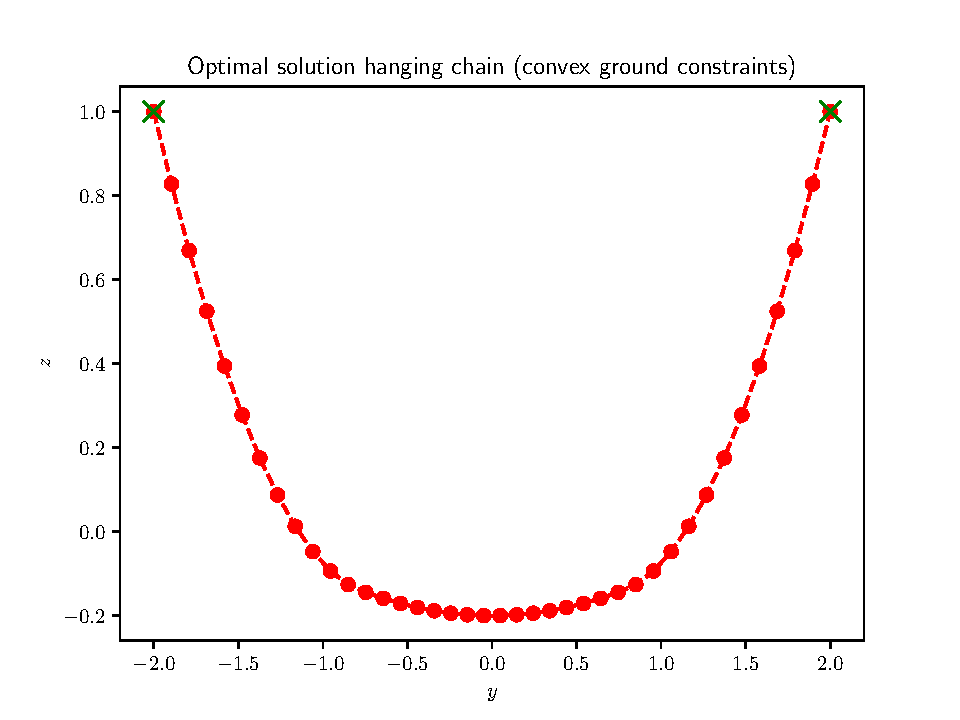
\includegraphics[width=\linewidth]{convex.pdf}
    \caption{Convex ground constraint $z_i\geq-0.2+0.1y_i^2$}
    \label{fig:conv}
  \end{subfigure}%
  \begin{subfigure}[t]{.5\textwidth}
    \centering
    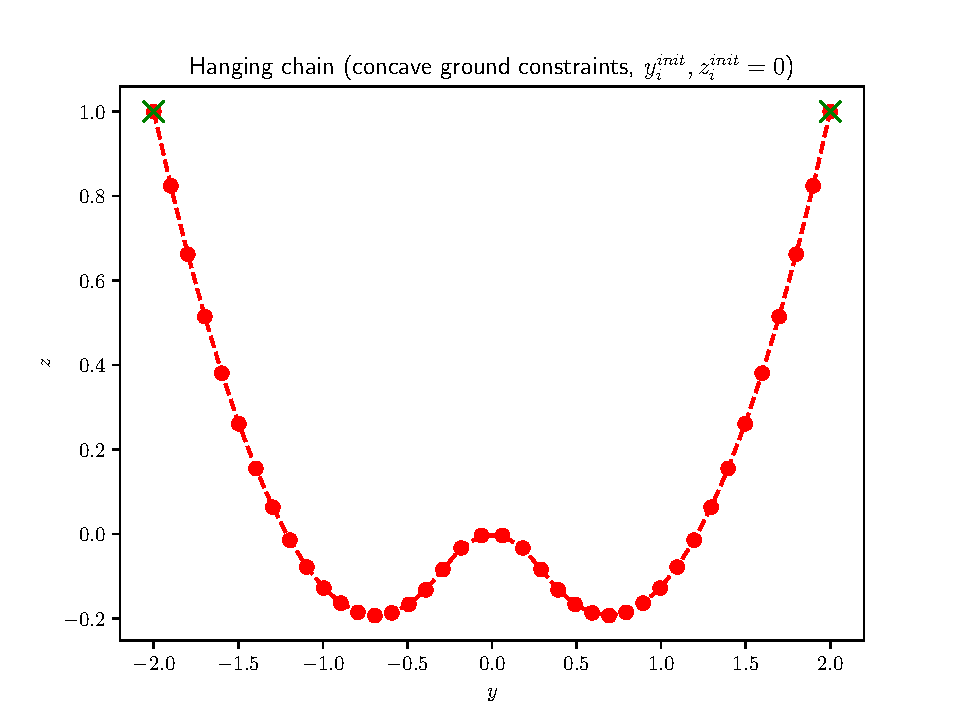
\includegraphics[width=\linewidth]{concave0.pdf}
    \caption{Concave ground constraint $z_i\geq-y_i^2$ \\with solver initialized at $y_i^{init}=z_i^{init}=0$}
    \label{fig:conc0}
  \end{subfigure}

  \begin{subfigure}[t]{.5\textwidth}
    \centering
    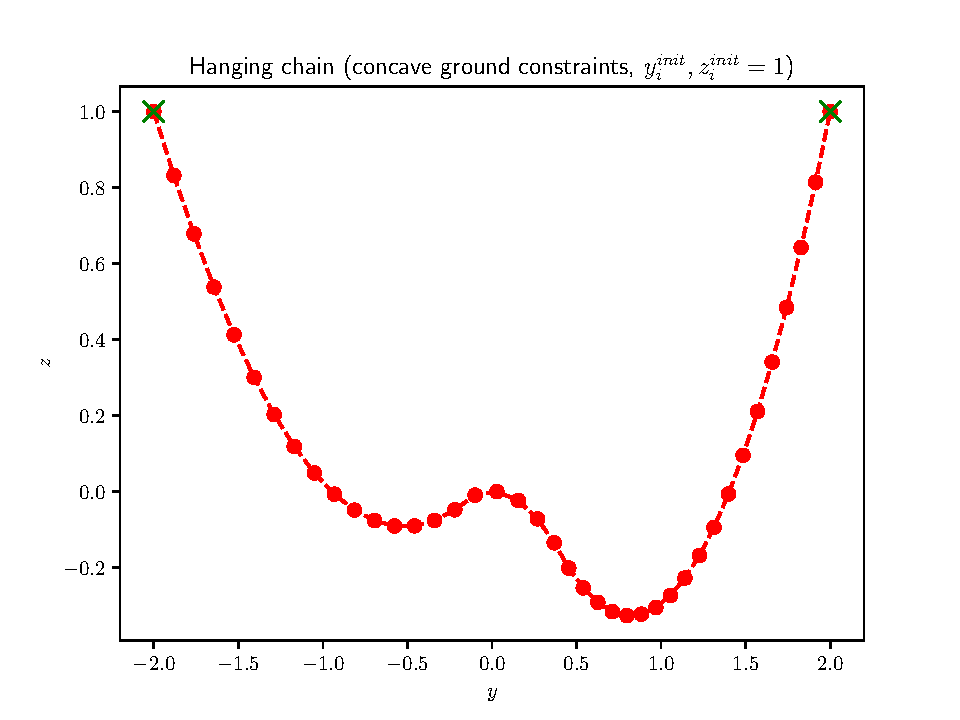
\includegraphics[width=\linewidth]{concave1.pdf}
    \caption{Concave ground constraint $z_i\geq-y_i^2$ \\with solver initialized at $y_i^{init}=z_i^{init}=1$}
    \label{fig:conc1}
  \end{subfigure}%
  \begin{subfigure}[t]{.5\textwidth}
    \centering
    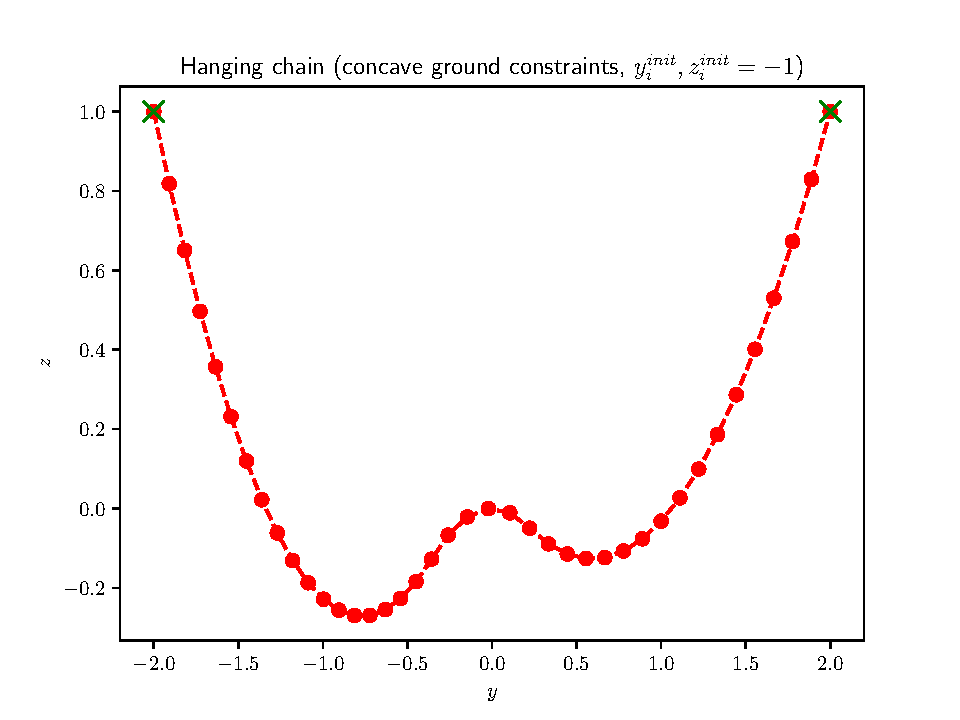
\includegraphics[width=\linewidth]{concave-1.pdf}
    \caption{Concave ground constraint $z_i\geq-y_i^2$ \\with solver initialized at $y_i^{init}=z_i^{init}=-1$}
    \label{fig:conc-1}
  \end{subfigure}
  \caption{Results for hanging chain energy minimization with differing inequality constraints, which form either a strictly convex problem with a unique solution (\autoref{fig:conv}) or a problem with concave constraints that have multiple local minima, which can be explored by altering the initial values of the decision variables in the solver (\autoref{fig:conc0}, \autoref{fig:conc1}, \autoref{fig:conc-1})}
  \label{fig:hanging-chain}
\end{figure}

\chapter{Minimum of a coercive function}
$\mathrm{Z\kern-.3em\raise-0.5ex\hbox{Z}}$: Let $f: \mathds{R}^n \to \mathds{R} \in C^0$ be a continuous, coercive function ($\lim_{\abss{x}\to\infty}f(x)=+\infty$), then there exists (at least) one global minimum.

\begin{itemize}
  \item Choose any point $\tilde{x}$, then choose any $y>f(\tilde{x})$
  \item Let $\Omega := \left\{ x \in \mathds{R}^n \middle| f(x) \leq y \right\}$ be the sublevel set of $f$ with respect to $y$, which is non-empty by construction since $\tilde{x}\in\Omega$
  \item $\Omega$ is bounded since $f$ is coercive and $\lim_{\abss{x}\to\infty}f(x)=+\infty$, there always exists a sphere of some radius $r$ around the origin $\vek{0}$ such that $\forall x \in \{x | \abss{x}\geq r\}: f(x) \geq y$, so the sphere bounds all points with function values lower than some given value, here $y$, and therefore the sublevel set $\Omega$
  \item $\Omega$ is closed since the sublevel set is defined through the inequality $\leq y$ (and not $<y$) and $f$ is continuous (so there is no open region due to discontinuities)
  \item $\Omega$ is closed, bounded and non-empty - therefore, by the Weierstrass theorem, there exists a minimizer $x^*\in\Omega$ of $f$ on $\Omega$
  \item By construction, $x^*$ is a minimizer of $f$ not only on $\Omega$ but on all of $\mathds{R}^n$, since $\Omega$ is a sublevel set and therefore $\forall x\in\mathds{R}^n\backslash \Omega: f(x) \geq y$ $\blacksquare$
\end{itemize}

\chapter{Lagrange duality and dual problems}
\section{Logarithmic barrier}
\begin{align*}
  p^* = \min_{x\in\mathds{R}^n}\quad &c^Tx-\sum_{j=1}^n \log x_j \\
  \text{s.t.}\quad  & a^Tx = b
\end{align*}
\begin{enumerate}
  \item \begin{align*}
    \mathcal{L}(x,\lambda) &= c^Tx-\sum_{j=1}^n \log x_j - \lambda^T \left(a^Tx - b\right)\\
    q(\lambda) &= \inf_{x\in\mathds{R}^n} \quad L(x,\lambda)\\
    &=  \inf_{x\in\mathds{R}^n} c^Tx-\sum_{j=1}^n \log x_j - \lambda^T \left(a^Tx - b\right)\\
    &=  \inf_{x\in\mathds{R}^n} -\sum_{j=1}^n \log x_j + c^Tx -\lambda^Ta^Tx + \lambda^Tb\\
    &=  \lambda^Tb + \inf_{x\in\mathds{R}^n} -\sum_{j=1}^n \log x_j + (c -\lambda a)^T x\\
    &=  \lambda^Tb + \inf_{x\in\mathds{R}^n} \underbrace{\sum_{j=1}^n \left((c -\lambda a)_j x_j -\log x_j \right)}_{=:k(x)}\\
    \frac{\partial k}{\partial x_j} &= (c_j - \lambda_j a_j) - \frac{1}{x_j} \overset{!}{=} 0\\
    \Longrightarrow x_j^* &\overset{!}{=} \frac{1}{c_j - \lambda_j a_j} &\textit{if $c_j-\lambda_j a_j > 0$ and $k(x)$ convex}\\
    q(\lambda) = \mathcal{L}(x^*, \lambda) &= \lambda^Tb + \sum_{j=1}^n \left(1 + \log (c_j - \lambda_j a_j)\right)\\
  \end{align*}
  so the dual problem is
  \begin{align*}
    d^* = \max_{\lambda\in\mathds{R}^n}\quad& n + \lambda^Tb + \sum_{j=1}^n \log (c_j - \lambda_j a_j)\\
    \text{s.t.}\quad& c-\lambda^T a > 0
  \end{align*}
  \item $d^* = p^*$ due to strong duality, since Slater's condition holds (affine equality constraints) and the primal problem is convex on $\mathds{R}^n_{++}$ (where solutions are feasible):
  \begin{align*}
    \frac{\partial}{\partial x_j} \left(c_j x_j - \log x_j\right) &= c_j - \frac{1}{x_j}\\
    \frac{\partial^2}{\partial x_j^2} \left(c_j x_j - \log x_j\right) &=  \frac{1}{x_j^2} \\
    \forall x_j \in\mathds{R}_{++}: \frac{1}{x_j^2} > 0
  \end{align*}
  % (if $\frac{1}{0^2}$ is defined to be $+\infty$ since $\frac{1}{x^2}$ approaches $+\infty$ from both sides, the primal problem is convex everywhere? Either way doesn't change $d^*=p^*$)
\end{enumerate}

\section{Linear programming}
\begin{enumerate}
  \item 
  \begin{align*}
    \min_{x\in\{0,1\}^n}\quad& -c^Tx \\
    \text{s.t.}\quad& Ax\geq b \\
  \end{align*}
  is equivalent to:
  \begin{align*}
    \min_{x\in\mathds{R}^n}\quad& -c^Tx \\
    \text{s.t.}\quad& Ax\geq b \\
    & x - x\otimes x  \\
  \end{align*}
  where $\otimes$ is component-wise multiplication and the equality constraint is equivalent to $\forall i\in\{1,\dots,n\}: x_i(1-x_i) = 0 \Longrightarrow x \in \{0,1\}^n$
  \item The reformulation is not convex, since the feasible set due to the equality constraints is still $\{0,1\}^n$ (intersected with some half-space defined by $Ax-b\geq 0$), which is not a convex set.
  \item $\mathcal{L}(x,\lambda,\mu) = -c^Tx -\lambda^T (x - x\otimes x) -\mu^T (Ax-b)$
  \item  \begin{align*}
    \frac{\partial }{\partial x} \mathcal{L}_i(x,\lambda,\mu) &= -c_i + \lambda_i (2x_i - 1) -(A^T\mu)_i \overset{!}{=} 0\\
    x_i^* &= \frac{c_i + (A^T\mu)_i}{2\lambda_i} + \frac{1}{2}\\
  \end{align*} for $\lambda_i \neq 0$, so the dual problem is: \begin{align*}
    \max_{\lambda,\mu} \br{\inf_x \mathcal{L}(x,\lambda,\mu)} &= \max_{\lambda,\mu} q(\lambda,\mu)\\ = \max_{\lambda,\mu} &= -c^Tx^* -\lambda^T (x^* - x^*\otimes x^*) -\mu^T (Ax^*-b)\\
    \text{s.t.}\, & \mu \geq 0 \\
    & \forall i: \lambda_i \neq 0 
  \end{align*}
  \item The dual problem is always convex (since $q(\lambda, \mu)$ is always concave by Theorem 4.3)
  \item Maximizing $q(\lambda, \mu)$ yields a lower bound to the ILP (Lemma 4.2), which could be used as the solution to the relaxed problem in a branch-and-bound approach to minimize the primal objective.
\end{enumerate}

\chapter{Fitting problems}
\section{Affine $L_2$ fitting}
\begin{enumerate}
  \item In matrix form, the least square problem can be denoted using $J\in\mathds{R}^{n\times 2}$: \[ J = \begin{bmatrix}
    x_1&1\\
    x_2&1\\
    \dots&\dots\\
    x_n&1
  \end{bmatrix} \]
  \item \begin{align*}
    \begin{bmatrix}\hat{a}\\\hat{b}\end{bmatrix} &= J^+ y = (J^T J)^{-1} J^T\\
    &= \br{
      \begin{bmatrix}x_1&x_2&\dots&x_n\\  1 & 1 & \dots & 1\end{bmatrix} 
      \begin{bmatrix}x_1&1\\x_2&1\\\dots&\dots\\x_n&1\end{bmatrix}
    }^{-1} 
    \begin{bmatrix}x_1&x_2&\dots&x_n\\  1 & 1 & \dots & 1\end{bmatrix} 
    \begin{bmatrix}y_1\\y_2\\\dots\\y_n\end{bmatrix}
    \\
    &= \begin{bmatrix}
      \sum_i x_i^2 & \sum_i x_i \\
      \sum_i x_i & n
    \end{bmatrix}^{-1}
    \begin{bmatrix}\sum_i x_i y_i\\ \sum_i y_i\end{bmatrix} 
    \\
    &= \br{n \begin{bmatrix}
      \overline{x^2} & \overline{x} \\
      \overline{x} & 1
    \end{bmatrix}}^{-1}
    n \begin{bmatrix}\overline{xy}\\ \overline{y}\end{bmatrix} 
    \\
    &= \frac{n}{n^2\br{\overline{x^2} - \overline{x}^2}} 
    \begin{bmatrix}
      1 & -\overline{x} \\
      -\overline{x} & \overline{x^2}
    \end{bmatrix}
    n \begin{bmatrix}\overline{xy}\\ \overline{y}\end{bmatrix} \\
    &= \frac{1}{\overline{x^2} - \overline{x}^2}  \begin{bmatrix}
      1 & -\overline{x} \\
      -\overline{x} & \overline{x^2}
    \end{bmatrix}
    \begin{bmatrix}\overline{xy}\\ \overline{y}\end{bmatrix} \\
    &= \frac{1}{\overline{x^2} - \overline{x}^2}  
    \begin{bmatrix}
      \overline{xy} -\overline{x}\cdot  \overline{y} \\
      - \overline{x}\cdot \overline{xy} + \overline{x^2} \cdot \overline{y}
    \end{bmatrix}
    \\
    \hat{a} &= \frac{\overline{xy} -\overline{x}\cdot  \overline{y}}{\overline{x^2} - \overline{x}^2}\\
    \hat{b} &= \frac{\overline{x^2} \cdot \overline{y}- \overline{x}\cdot \overline{xy}}{\overline{x^2} - \overline{x}^2} \\
  \end{align*}
  \item For fitting results see \autoref{fig:linreg} and fit with outliers in \autoref{fig:linregout}
\end{enumerate}

\section{Affine $L_1$ fitting}
\begin{enumerate}
  \item \begin{align*}
    \min_{a,b\in\mathds{R}, s\in\mathds{R}^n} &\sum_{i=1}^{N} s_i \\
    \text{s.t.}\quad  &s_i + (a x_i + b - y_i) \geq 0 \quad\forall i\in\mathds{N}_1^N\\
                      &s_i - (a x_i + b - y_i) \geq 0 \quad\forall i\in\mathds{N}_1^N\\
  \end{align*}
  since the constraints imply $s_i \geq \abs{a x_i + b - y_i}$ and therefore each $s_i$ is an upper bound to the problem. As the slack variables are minimized, so is the L1 norm of the residuals.
  \item For fitting results see \autoref{fig:linregl1} and fit with outliers in \autoref{fig:linregoutl1}
  \item While the L2 norm seems to perform better in the absence of outliers, giving a more accurate estimation of the true function parameters, the L1 fit is much more robust to outliers.
\end{enumerate}


\begin{figure}[H]
  \begin{subfigure}{0.5\textwidth}
    \centering
    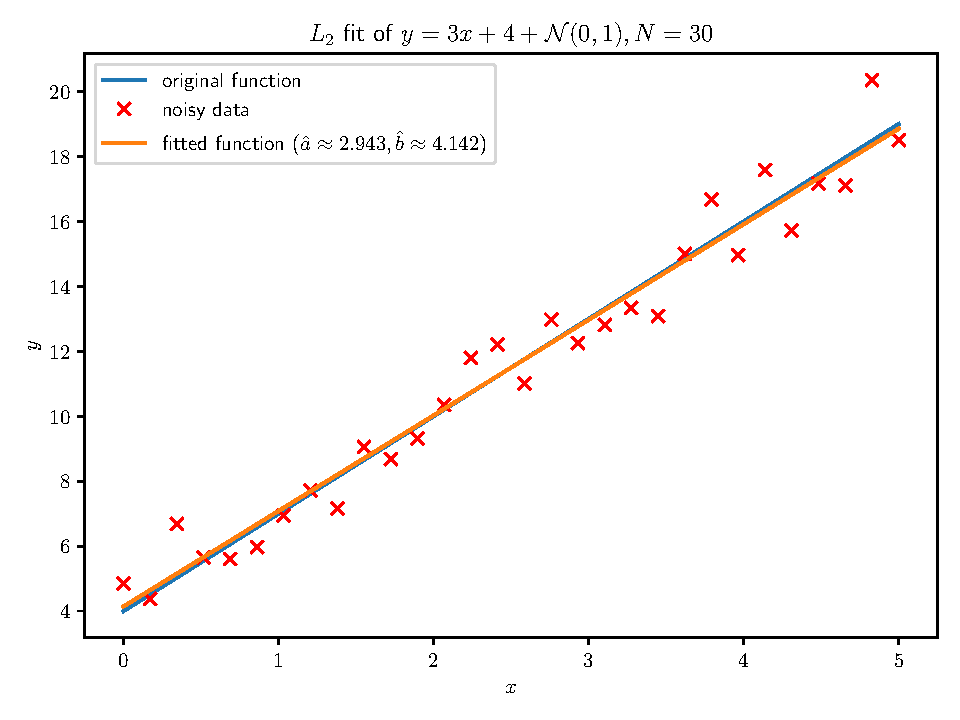
\includegraphics[width=\linewidth]{linreg.pdf}
    \caption{$L_2$ fit to noisy data}
    \label{fig:linreg}
  \end{subfigure}%
  \begin{subfigure}{0.5\textwidth}
    \centering
    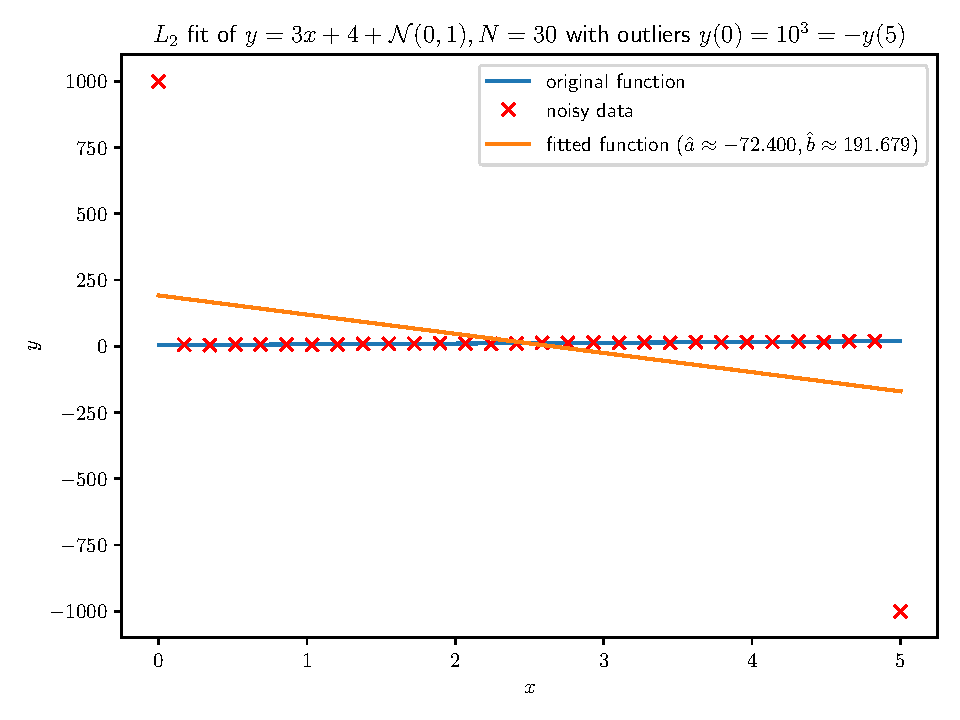
\includegraphics[width=\linewidth]{linregout.pdf}
    \caption{$L_2$ fit with outliers}
    \label{fig:linregout}
  \end{subfigure}

  \begin{subfigure}{0.5\textwidth}
    \centering
    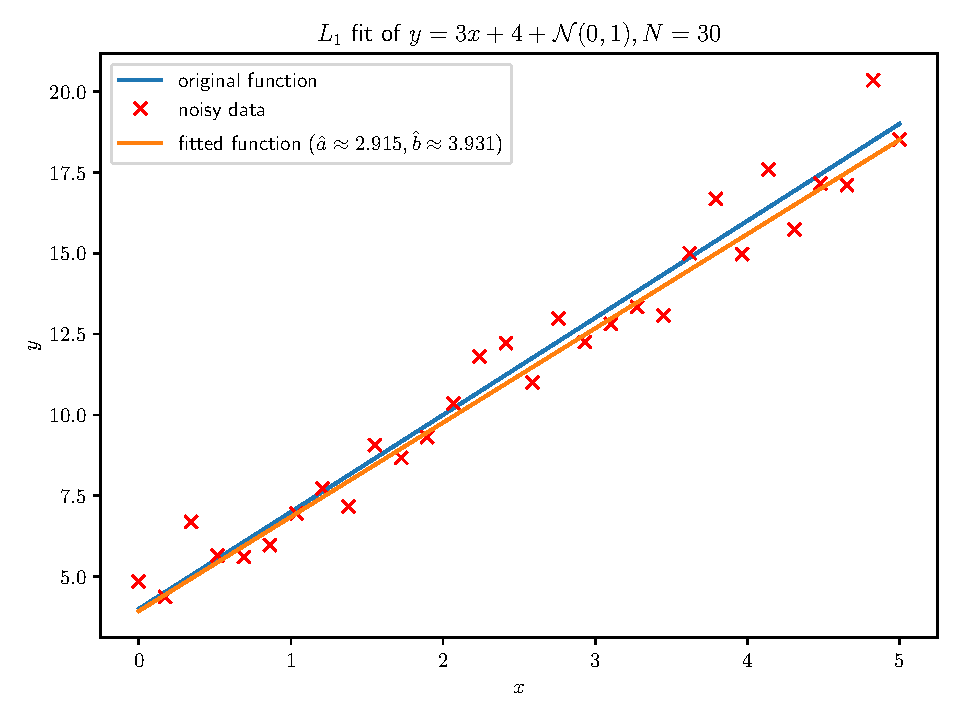
\includegraphics[width=\linewidth]{linregl1.pdf}
    \caption{$L_1$ fit to noisy data}
    \label{fig:linregl1}
  \end{subfigure}%
  \begin{subfigure}{0.5\textwidth}
    \centering
    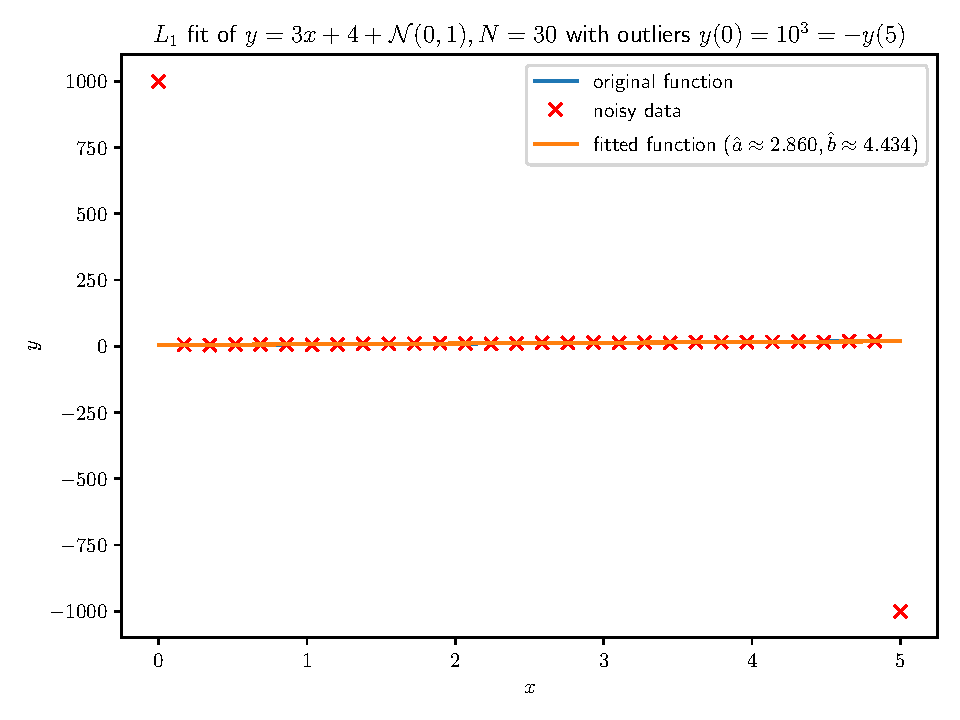
\includegraphics[width=\linewidth]{linregoutl1.pdf}
    \caption{$L_1$ fit with outliers}
    \label{fig:linregoutl1}
  \end{subfigure}

\end{figure}


\section{Regularized linear least squares}
\begin{enumerate}
  \item \begin{align*}
    f(x) &= \frac{1}{2} \abss{y - Jx}_2^2 + \frac{\alpha}{2}x^T Q x\\
    \nabla f(x) &= J^T J x - J^T\eta + \alpha Q x\\
    \nabla^2 f(x) &= J^T J + \alpha Q\\
  \end{align*}
  so since $Q\succ 0$ the solution is unique ($\nabla^2f(x)\succ 0$) if either $\alpha>0$ or $J$ is full column-rank and therefore the Gram matrix has $J^T J\succ 0$. If any of the two matrices $J^T J$ and $\alpha Q$ is positive definite, then since the other is at least positive semidefinite, the result of the summation must be positive definite.
  \item \begin{align*}
  \nabla f(x) = J^T J x - J^T\eta + \alpha Q x &\overset{!}{=} 0\\
  (J^T J + \alpha Q) x &= J^T\eta\\
  x^*(\alpha) &= (J^T J + \alpha Q)^{-1} J^T\eta\\
  \end{align*}
  \item \begin{align*}
    x^T Q x &\overset{!}{=} \abss{\tilde{x}}_2^2\\
    &= x^T B B x &\text{let $B=\sqrt{Q}\succ 0$ the unique principal square root}\\
    &= x^T B^T B x &B = B^T \text{since $Q,B$ symmetric}\\
    &= (B x)^T B x &\\
    &= \abss{B x}_2^2 &\\
    \Longrightarrow \tilde{x} &= Bx\\
  \end{align*}
  and therefore:
  \begin{align*}
    \tilde{J}\tilde{x} &\overset{!}{=} J x \\
    \tilde{J}B x &= J x &\text{insert $\tilde{x} = Bx$} \\
    \tilde{J}B &= J\\
    \Longrightarrow \tilde{J} &= J \br{B^{-1}} &\text{$B^{-1}$ exists since $Q\succ 0\Longrightarrow B B \succ 0 \Longrightarrow B \succ 0$}\\
  \end{align*}
  \item $x^*(\alpha) = \br{\tilde{J}^T\tilde{J} + \epsilon \mathds{1}}^{-1} \tilde{J}^T y$ as shown in the previous exercise, so by Lemma 6.1 it follows that for $\alpha \to 0$ it holds that $x^*(\alpha) = \tilde{J}^+ y$ where $\tilde{J}^+$ is the Moore-Penrose inverse. Since that expression has no dependence on $\alpha$, it follows trivially that $\lim_{\alpha\to 0} x^*(\alpha) = \tilde{J}^+ y$, meaning $x^*$ converges to the vector $\tilde{J}^+ y$.
  \item Since the Moore-Penrose pseudo inverse yields the unique solution to the problem: \begin{align*}
    x^* = \tilde{J}^+ y  = J^+ y= \min_{x\in\mathds{R}^n} &\frac{1}{2}\abss{x}_2^2\\
    \text{s.t.}\quad &x\in\mathcal{S}^*
  \end{align*}
  where $S^*=\left\{x \,\middle|\, \nabla \br{\frac{1}{2} \abss{y - Jx}_2^2} = \vek{0}\right\}$ then due to the constraint the solution $x^*$ yielded by $x^*=\tilde{J}^+ y$ is an element of the solution set $\mathcal{S}^*$ of the unregularized minimization problem (namely that of least $L_2$ magnitude). Note that $\lim_{\alpha\to 0} \tilde{J} = J$.
\end{enumerate}

\chapter{Source Code}
\section{Hanging Chain}
\inputminted{python}{ex2_hanging_chain.py}
\section{Regression}
\inputminted{python}{ex2_linreg.py}

\end{document}